
\section{Mathematische Grundlagen}
\label{chap:Style}

\subsection{Koordinatensysteme}

Häufig sind wir daran interessiert, geometrische Dinge in der Mathematik darzustellen um mit ihnen zu rechnen. \\
Um mit mathematischen Mitteln geometrische Probleme beschreiben zu können, müssen wir ein System einführen, wie wir
Positionen im Raum und Richtungen charakterisieren können. \\
Zu diesem Zweck werden \textbf{Koordinatensysteme} eingeführt.

\definition{Koordinatensystem}
\beginip
Ein Koordinatensystem dient zur eindeutigen Bezeichnung der Position von Punkten in einem geometrischen Raum.  \\
Befinden wir uns in einem 3-Dimensionalem Raum so werden 3 \textbf{Basisvektoren} benötigt, um jeden Punkt im Raum eindeutig zu definieren. \\
Möchten wir nun einen Punkt im Raum beschreiben, so müssen wir zuerst einen Punkt im Raum als Bezugspunkt (Ursprung) definieren. \\
Danach beschreiben wir den gesuchten Punkt als \textbf{Linearkombination} der Basisvektoren. Die Koeffizienten der Linearkombination bezeichnen wir dabei als Koordinaten.
\iend


\bsptask{Beispiel}{Punkt im Koordinatensystem}
\beginbsp
Geben sie die Koordinaten des folgenden Punktes P im 2 Dimensionalen an. \\ Als Basisvektoren verwenden wir die Vektoren: $ \vec{e}_1, \vec{e}_2$
\begin{center}
	\ibox{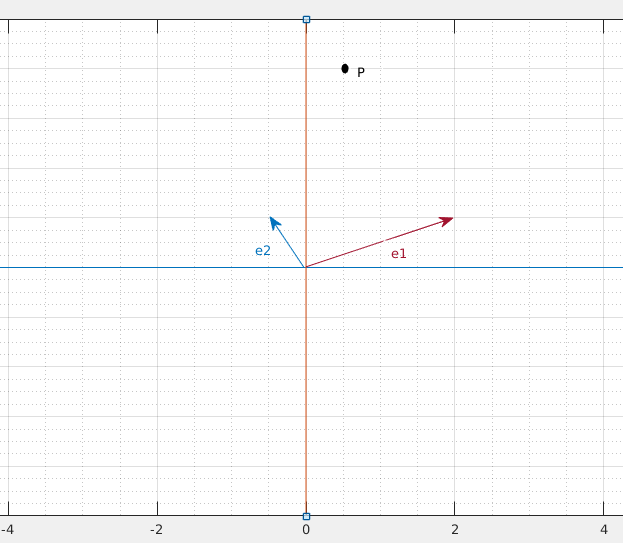
\includegraphics[scale=2.0]{img/bsp1_coord.png}}
\end{center}
\iend
\newpage
\bsp{Lösung}{}
\beginbsp
Um vom Ursprung den Punkt P mit den Basisvektoren $\vec{e}_1$ und $\vec{e}_2$ zu erreichen, müssen die Vektoren wie folgt kombiniert werden:
\begin{center}
	\ibox{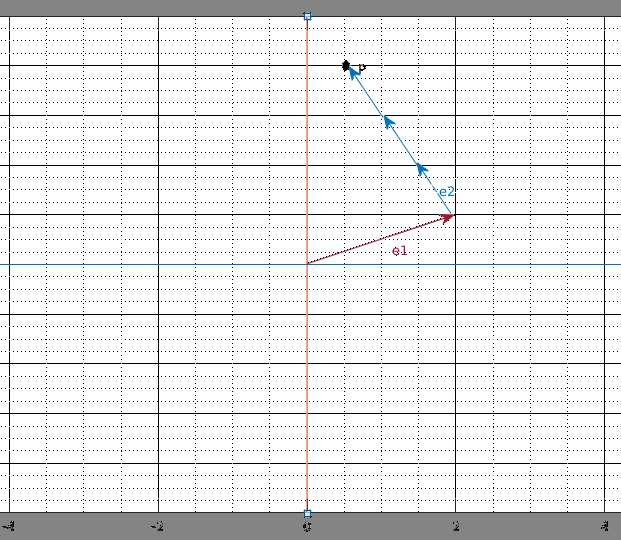
\includegraphics[scale=2.0]{img/sol_1_koord.png}}
\end{center}
Somit gilt für den Punkt P : \\
\begin{center}
	$\vec{P} = 1\cdot \vec{e}_1 + 3 \cdot \vec{e}_2$ \\
	$\rightarrow \doubleunderline{ P = \left ( \begin{array}{c} 1 \\ 3 \end{array}\right)}$
\end{center}
\iend

\newpage


\important{Konzept}{Winkelabhängige Basisvektoren *}
\beginip
In gewissen Koordinatensystemen werden Basisvektoren verwendet, dessen Richtung sich Abhängig  des Winkels ändern. \\
Sie werden dazu verwendet, Punkte im Raum abhängig eines Winkels zu beschreiben. \\
\textbf{Der Basisvektor zeigt dabei immer in die Richtung des Winkels} \\
\\
* Dies ist ein Konzept, welches Mathematisch nicht genau so existiert.
\iend

\bsptask{Beispiel}{Punkt im Koordinatensystem - Polarkoordinaten}
\beginbsp
Geben sie die Koordinaten des folgenden Punktes P im 2 Dimensionalen an.
\\
Als Basisvektoren verwenden wir die Vektoren: $ \vec{e}_1, \vec{e}_2$, wobei $\vec{e}_2$ ein Winkelabhängiger Basisvektor ist.
\begin{center}
	\ibox{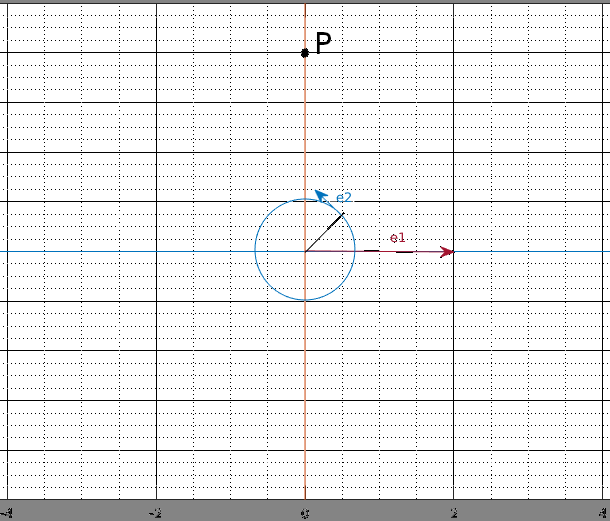
\includegraphics[scale=2.0]{img/ex2_coord.png}}

\end{center}
\iend
\bsp{Lösung}{}
\beginbsp
Da der Punkt P einen Winkel von $90^\circ = \frac{\pi}{2}$ einschliesst, müssen wir ein Winkelabhängigen Basisvektor $\vec{e}_2$ mit $\frac{\pi}{2}$ multiplizieren. \\
Der Abstand des Punktes zum Ursprung beträgt 8 Einheiten, wobei der Vektor $\vec{e}_1$ die Länge von 2 Einheiten besitzt. \\
Somit gilt für die Koordinaten des Punktes P in Abhängigkeit von $\vec{e}_1 , \vec{e}_2$:
\begin{center}
	$\vec{P} = \frac{\pi}{2} \cdot \vec{e}_2 + 4\cdot \vec{e}_1$
	\\ $\displaystyle \doubleunderline{P = \left ( \begin{array}{c} 4 \\ \frac{\pi}{2} \end{array}\right)}$
\end{center}

\iend
\newpage




	\subsubsection{Kartesische Koordinaten}

	\important{Kartesische Koordinaten} {}
	\beginip
	Kartesische Koordinaten werden als bekannt vorausgesetzt. \\
	Kartesische Koord. werden vor allem dann verwendet, wenn die geometrische Anordnung \textbf{Symmetrien bezüglich einer Ebene} besitzt.
	\begin{center}
		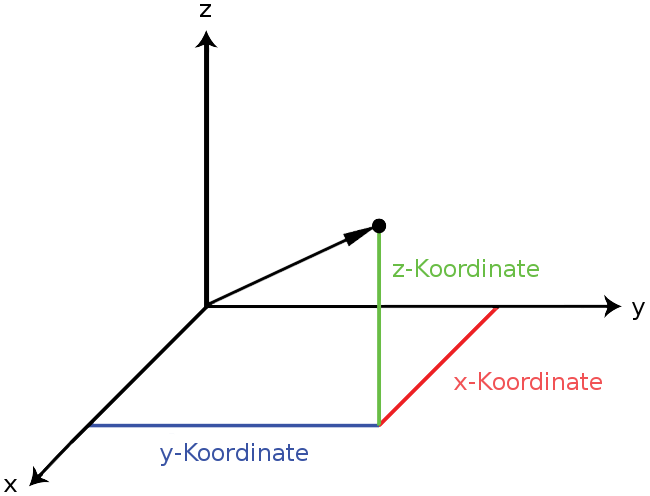
\includegraphics[scale=0.3]{img/cartesian.png}
	\end{center}
	\iend

	\newpage
%TODO ggf. Zusammenfassung

	\subsubsection{Zylinderkoordinaten}

\important{Zylinderkoordinaten} {}
\beginip
Zylinderkoordinaten werden meist dann
verwendet, wenn die geometrischen Anordnung Symmetrien bezüglich einer \textbf{Gerade} aufweist. \\
Zylinderkoordinaten besitzen 3 Basisvektoren wovon 1 winkelförmig ist. \\
\\
\textbf{Basisvektoren}
\begin{enumerate}
	\item $\vec{e}_\rho$ Beschreibt den Abstand zur Symmetrieachse
	\item $\vec{e}_\varphi$ Beschreibt den Winkel des Punktes in der XY-Ebene
	\item $\vec{e}_z$ Beschreibt den Abstand auf der Symmetrieachse
\end{enumerate}
\begin{center}
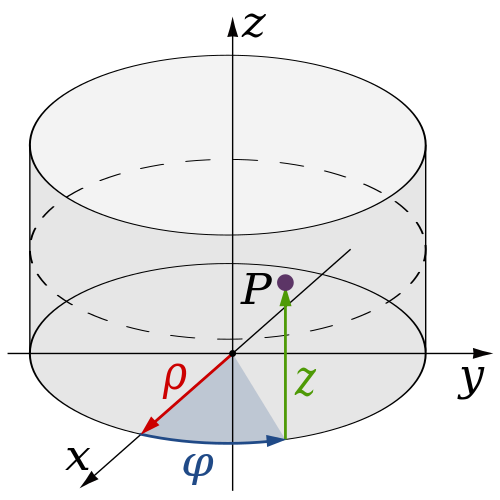
\includegraphics[scale = 0.4]{zylinderkoord.png}
\end{center}


\iend
\newpage
\important{Richtung der einzelnen Basisvektoren für beliebige Punkte im Raum: }{}


\beginip


\fboxsep=0pt
\begin{minipage}[t]{0.48\linewidth}

	\begin{center}

		\textbf{Radialer Vektor} $\vec{e}_\rho$

	\end{center}

	\begin{center}

		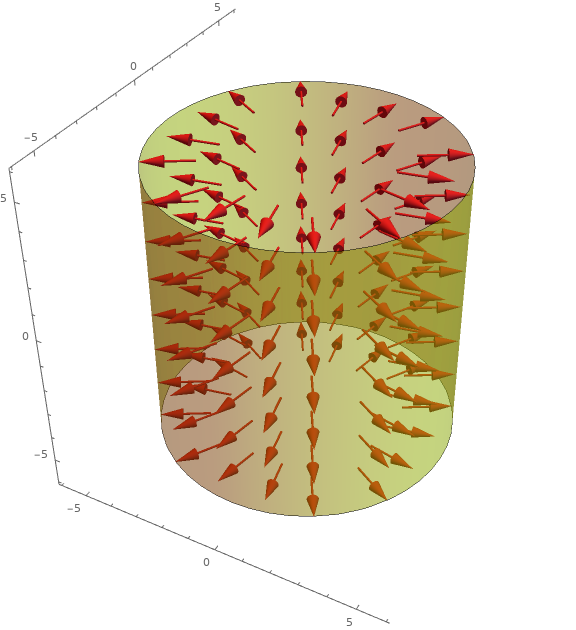
\includegraphics[scale=0.3]{zylindric_rho.png}

	\end{center}
\end{minipage}
\hfill%
\begin{minipage}[t]{0.48\linewidth}



	\begin{center}

		\textbf{Azimutaler Vektor} $\vec{e}_\varphi$

	\end{center}

	\begin{center}

			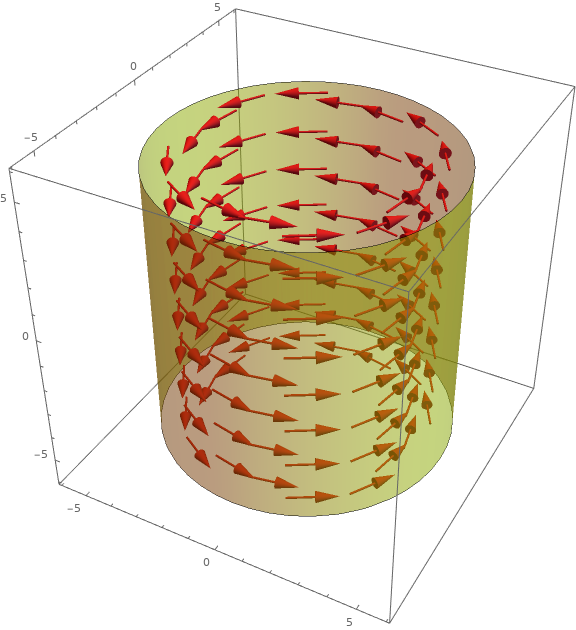
\includegraphics[scale=0.3]{zylindric_phi.png}


	\end{center}

\end{minipage}


\begin{center}

	\textbf{Abstandsvektor} $\vec{e}_z$

\end{center}

\begin{center}

		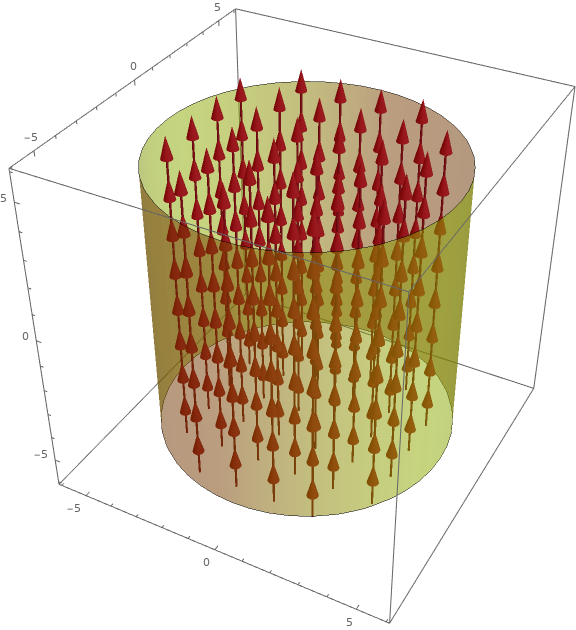
\includegraphics[scale=0.3]{zylindric_z.png}

\end{center}
\iend



\newpage

	\subsubsection{Kugelkoordinaten}

\important{Kugelkoordinaten} {}
\beginip
Kugelkoordinaten werden meist dann verwendet, wenn die geometrischen Anordnung \textbf{Punktsymmetrien} aufweist. \\
Kugelkoordinaten besitzen 3 Basisvektoren wovon 2 winkelabhängig sind. \\
\\
\textbf{Basisvektoren}
\begin{enumerate}
	\item $\vec{e}_r$ Beschreibt den Abstand zum Ursprung
	\item $\vec{e}_\theta$ Beschreibt den Winkel des Punktes in der ZY-Ebene
	\item $\vec{e}_\varphi$ Beschreibt den Winkel des Punktes in der XY-Ebene
\end{enumerate}
\begin{center}
	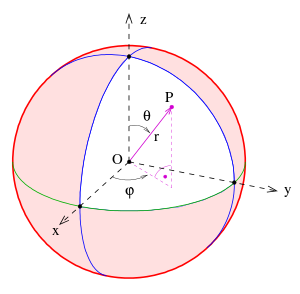
\includegraphics[scale = 0.5	]{kugelkoord.png}
\end{center}


\iend
\newpage
\important{Richtung der einzelnen Basisvektoren für beliebige Punkte im Raum: }{}


\beginip


\fboxsep=0pt
\begin{minipage}[t]{0.48\linewidth}

	\begin{center}

		\textbf{Radialer Vektor} $\vec{e}_r$

	\end{center}

	\begin{center}

		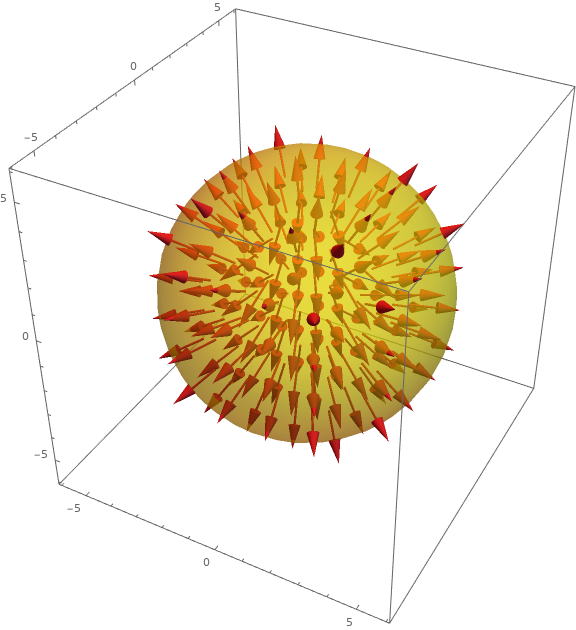
\includegraphics[scale=0.4]{spherical_r.png}

	\end{center}
\end{minipage}
\hfill%
\begin{minipage}[t]{0.48\linewidth}



	\begin{center}

		\textbf{Azimutaler Vektor} $\vec{e}_\varphi$

	\end{center}

	\begin{center}

		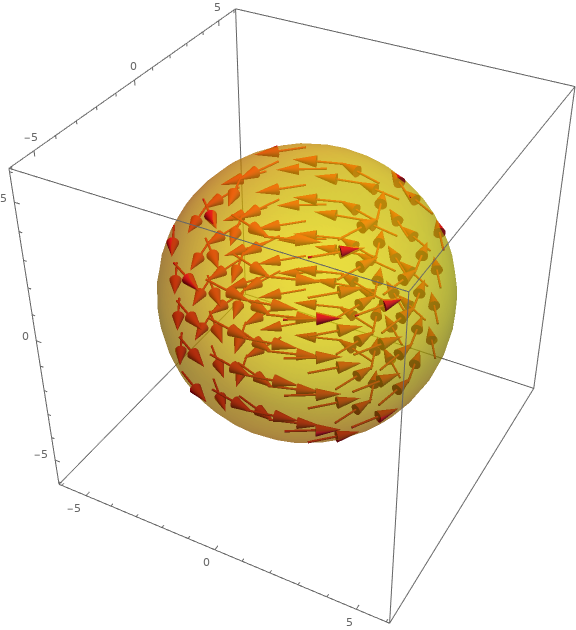
\includegraphics[scale=0.4]{spherical_phi.png}

	\end{center}

\end{minipage}


\begin{center}

	\textbf{Meridonaler Vektor} $\vec{e}_\theta$

\end{center}

\begin{center}

	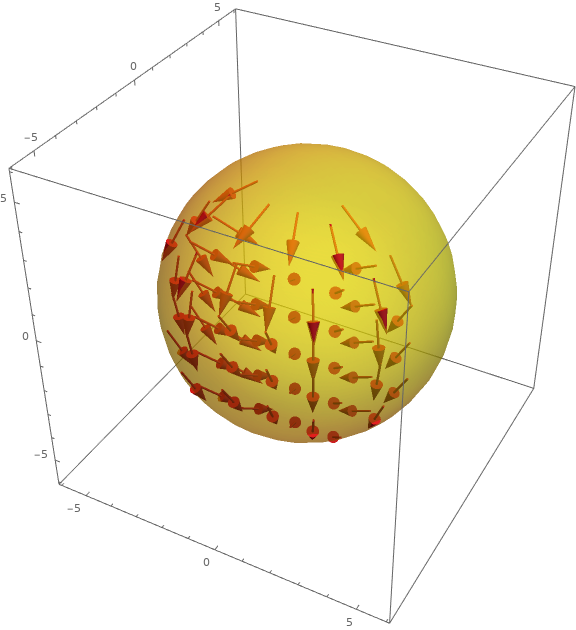
\includegraphics[scale=0.4]{spherical_theta.png}

\end{center}

% \formulaBegin
% $\displaystyle \vec{F}(r, \theta, \varphi) = \left(\begin{array}{c} 1 \\ 0 \\ 0 \end{array}\right)_{K} = 1 \cdot \vec{e}_r$ \\
%
% \formulaEnd


% \formulaBegin
% $\vec{F}(r, \theta, \varphi) = \left(\begin{array}{c} 0 \\ 1 \\ 0 \end{array}\right)_{Kugel\ Koordinaten} = 1 \cdot \vec{e}_\theta$ \\
%
% \formulaEnd

%
% \formulaBegin
% $\vec{F}(r, \theta, \varphi) = \left(\begin{array}{c} 0 \\ 0 \\ 1 \end{array}\right)_{Kugel\ Koordinaten} = 1 \cdot \vec{e}_\varphi$ \\
%
% \formulaEnd





\iend

\newpage
\subsubsection{Zusammenfassung}
\bgroup

\begin{tabular}{ c | c | c }
  Kartesische Koordinaten & Zylinderkoordinaten & Kugelkoordinaten \\
	\hline
		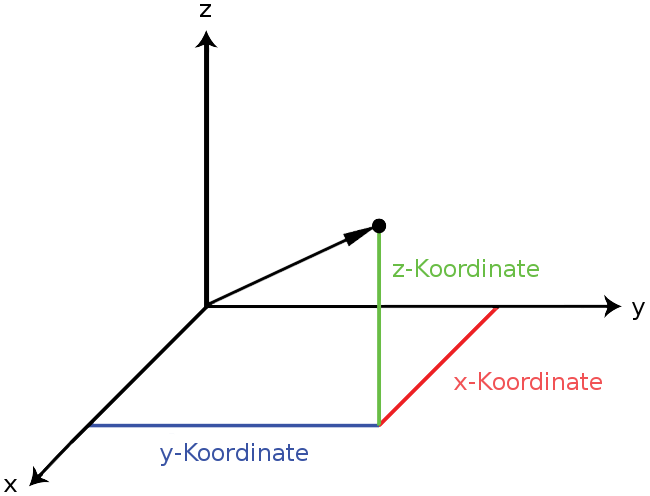
\includegraphics[width = 0.25\columnwidth]{img/cartesian.png} &
	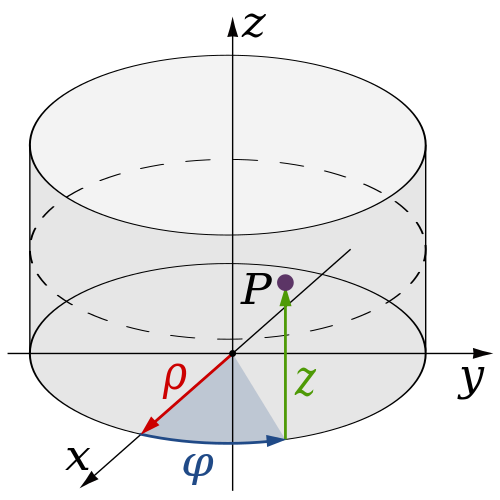
\includegraphics[width = 0.25\columnwidth]{zylinderkoord.png} &  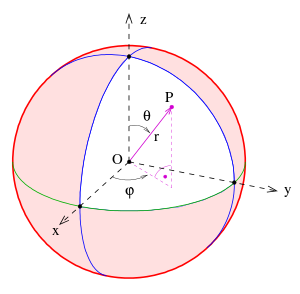
\includegraphics[width = 0.25\columnwidth]{kugelkoord.png} \\
	\hline
 \textbf{Anwenden bei:}& \textbf{Anwenden bei:} &  \textbf{Anwenden bei:}\\
 Symmetrie zu Ebene & Symmetrie zu Achse & Symmetrie zu Punkt \\
 \hline
   $\displaystyle \left ( \begin{array}{c} x \\ y \\ z  \end{array}\right)} = x \cdot \vec{e}_x + y \cdot \vec{e}_y + z \cdot \vec{e}_z$ &

	$\displaystyle \left ( \begin{array}{c} \rho \\ \varphi \\ z  \end{array}\right)} = \rho \cdot \vec{e}_\rho + \varphi \cdot \vec{e}_\varphi + z \cdot \vec{e}_z$ &



		$\displaystyle \left ( \begin{array}{c} r \\ \theta \\ \varphi  \end{array}\right)} = r \cdot \vec{e}_r + \theta \cdot \vec{e}_\theta + \varphi \cdot \vec{e}_\varphi $  \\
		\hline
			 $\vec{e}_x$  &  $\vec{e}_\rho$  &  $\vec{e}_r$ \\
			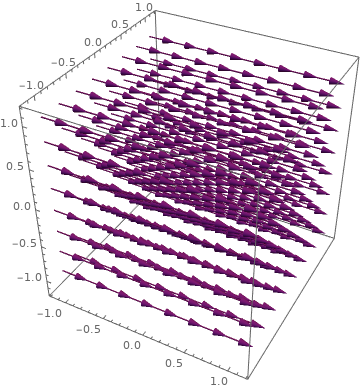
\includegraphics[width=0.25\columnwidth]{img/kart_x.png}

			&

			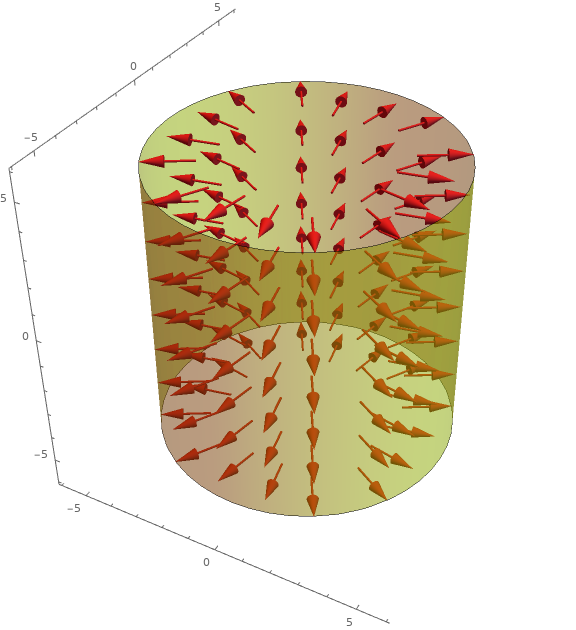
\includegraphics[width=0.25\columnwidth]{zylindric_rho.png}  & 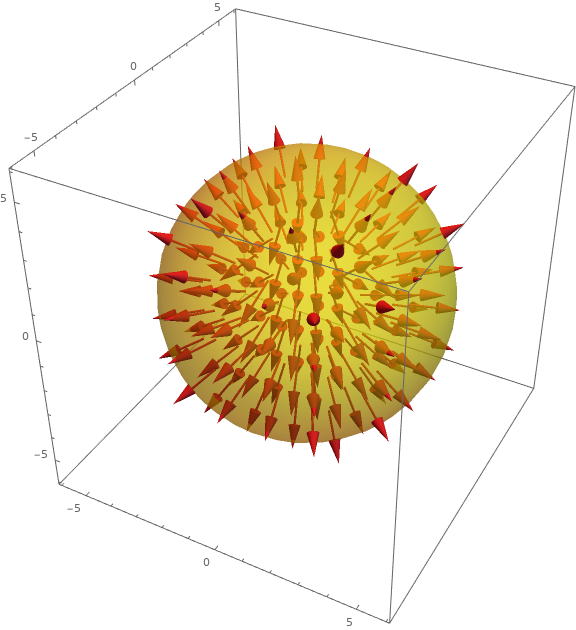
\includegraphics[width=0.25\columnwidth]{spherical_r.png} \\

			\hline
				 $\vec{e}_y$  &  $\vec{e}_\varphi$  &  $\vec{e}_\theta$ \\

			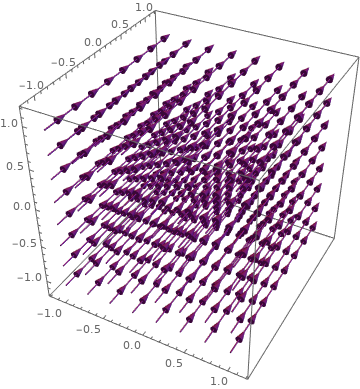
\includegraphics[width=0.25\columnwidth]{img/kart_y.png} & 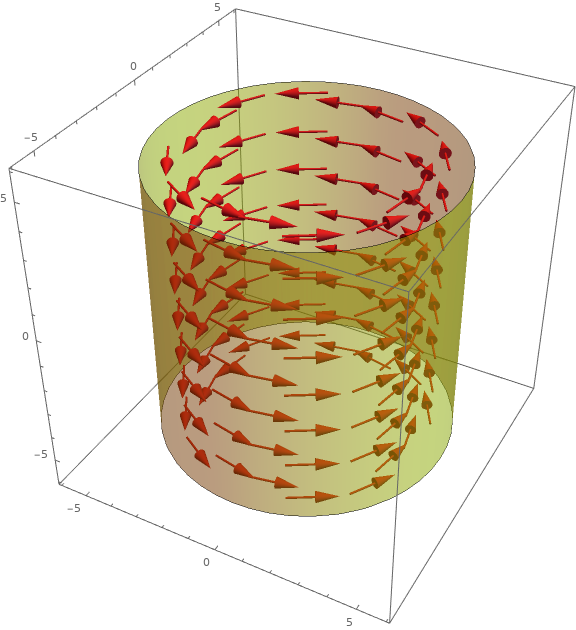
\includegraphics[width=0.25\columnwidth]{zylindric_phi.png}  &  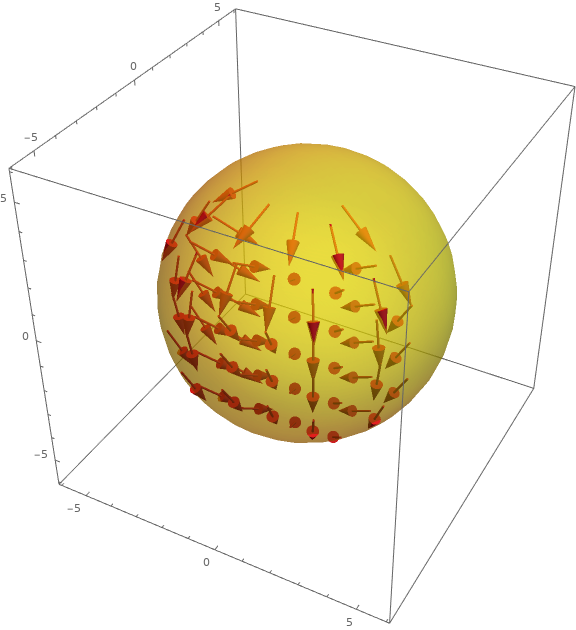
\includegraphics[width=0.25\columnwidth]{spherical_theta.png} \\
			\hline
				 $\vec{e}_z$  &  $\vec{e}_z$  &  $\vec{e}_\varphi$ \\
			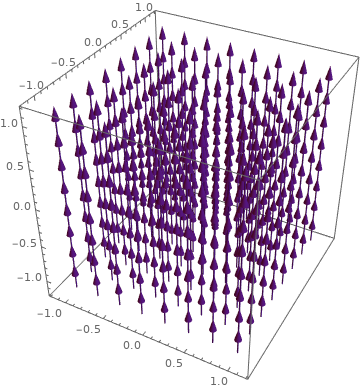
\includegraphics[width=0.25\columnwidth]{img/kart_z.png} & 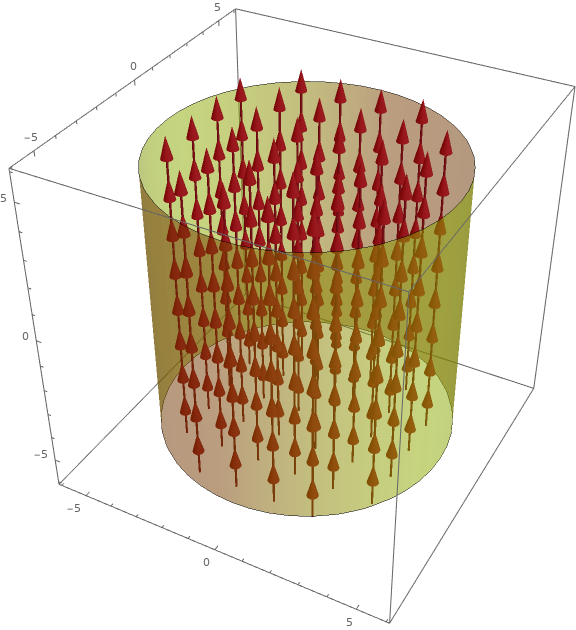
\includegraphics[width=0.25\columnwidth]{zylindric_z.png}  &  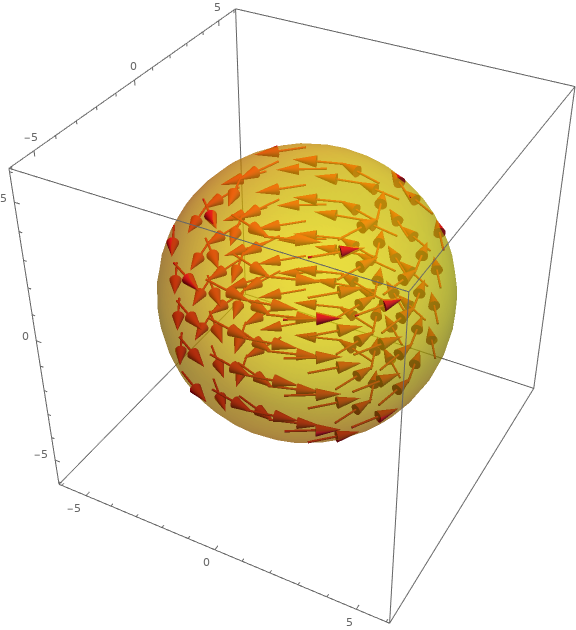
\includegraphics[width=0.25\columnwidth]{spherical_phi.png} \\
			\hline

\end{tabular}
\egroup

\newpage






\subsection{Vektorfelder}
Möchten wir eine physikalische Grösse im Raum beschreiben, so sind wir häufig nicht nur an den ortsabhängigen Punkten interessiert. \\
Meistens möchten wir jedem Punkt im Raum eine Richtung zuordnen. \\
Möchten wir beispielsweise die Erdanziehungskraft modellieren, so wollen wir jedem Punkt im Raum einen \textbf{Vektor} zuweisen, der in Richtung der Kraftwirkung zeigt. \\
Seine Länge soll zudem die Information beinhalten, wie stark die Kraft an diesem Punkt wirkt.










%
%
%
% \formulaBegin
% $\vec{F}(\rho, \varphi, z) = \left(\begin{array}{c} 1 \\ 0 \\ 0 \end{array}\right)_{Zylinder\ Koordinaten} = 1 \cdot \vec{e}_\rho$ \\
%
% \formulaEnd
% \begin{center}
%
% 	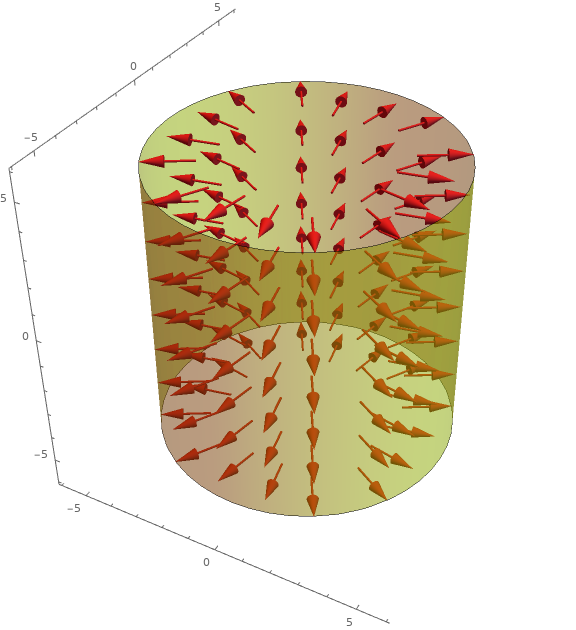
\includegraphics[scale=0.4]{zylindric_rho.png}
%
% \end{center}
%
%
% \formulaBegin
% $\vec{F}(\rho, \varphi, z) = \left(\begin{array}{c} 0 \\ 1 \\ 0 \end{array}\right)_{Zylinder\ Koordinaten} = 1 \cdot \vec{e}_\varphi$ \\
%
% \formulaEnd
% \begin{center}
%
% 	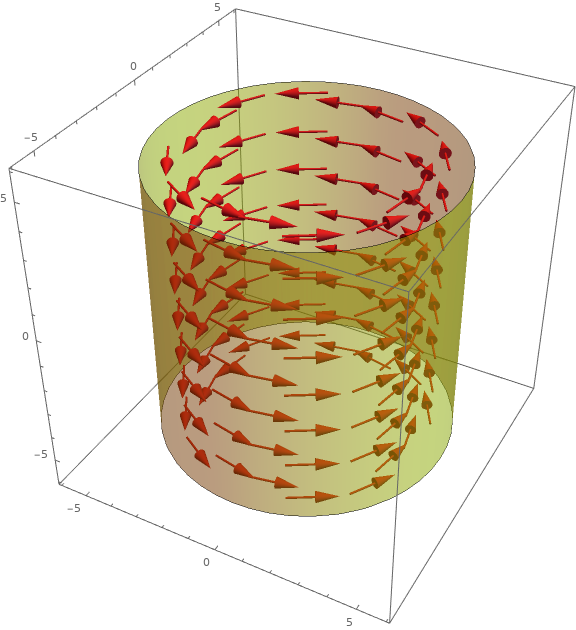
\includegraphics[scale=0.4]{zylindric_phi.png}
%
% \end{center}
%
%
%
%
% \formulaBegin
% $\vec{F}(\rho, \varphi, z) = \left(\begin{array}{c} 0 \\ 0 \\ 1 \end{array}\right)_{Zylinder\ Koordinaten} = 1 \cdot \vec{e}_z$ \\
%
% \formulaEnd
% \begin{center}
%
% 	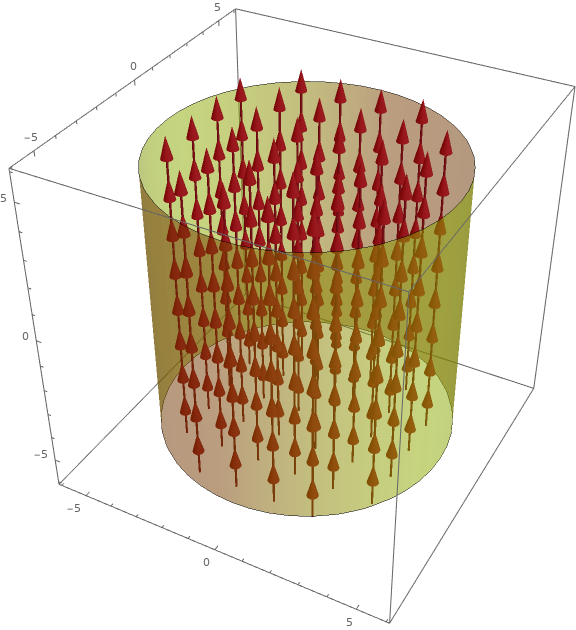
\includegraphics[scale=0.4]{zylindric_z.png}
%
% \end{center}
%
%
%
% \important{Zylinderkoordinaten} {}
% \beginip
%
% 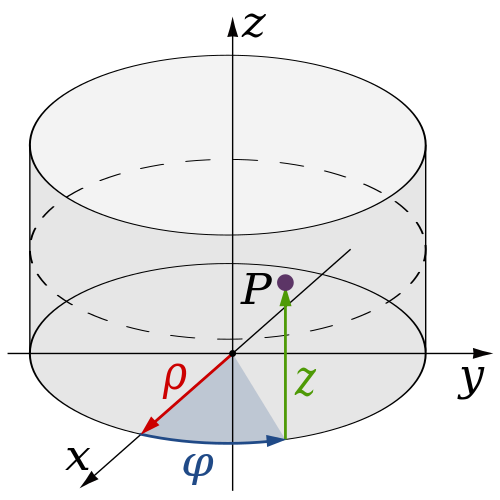
\includegraphics[scale = 0.4]{zylinderkoord.png}
% \iend
%
% \important{Kugelkoordinaten} {}
% \beginip
% \iend
%

\important{Defintion}{Vektorfeld}
\beginip
Ein Vektorfeld, bezeichnet eine mathematische Funktion, welche anstatt einer skalaren Grösse Vektoren zurück gibt. \\
Häufig ist ein Vektorfeld nicht nur von einer Variable (x) abhängig, sondern besitzt 3 Parameter (x,y,z) die wir manchmal als Ortsvektor $\vec{r}$ zusammenfassen.  \\
\iend

\bsp{Beispiel} {Vektorfeld - Gravitation}

\beginbsp
Möchten wir beispielsweise das Gravitationsfeld der Erde mathematisch beschreiben, würden wir dies in Form eines Vektorfeldes tun. \\
Dieses Vektorfeld soll jedem Punkt einen Kraftvektor zuweisen, welcher in Richtung Erdmittelpunkt zeigt. \\
Da die Erde punktsymmetrisch ist, ist es sinnvoll Kugelkoordinaten zu verwenden. \\
Die Stärke der Gravitationskraft auf ein Massepunkt der Masse m ist definiert als:
\begin{center}
	$F_M = \frac{M \cdot G}{r^2}$
\end{center}

Somit folgt für das Vektorfeld, das die Gravitationskraft beschreibt:
\begin{center}
	$\displaystyle \vec{F}_M (r,\theta,\varphi) = \frac{M \cdot G}{r^2} \cdot (- \vec{e}_r)$
\end{center}

\begin{center}
	\ibox{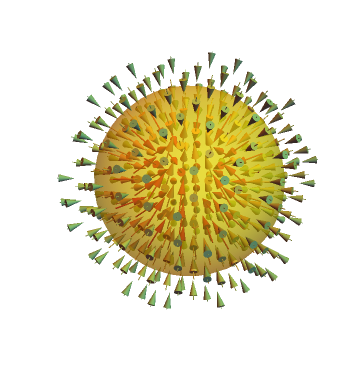
\includegraphics[scale=0.4]{img/vektorfeld-g.png}}

\end{center}
\iend

\newpage
\subsection{Weg- und Oberflächenintegrale}

\gl{Gleichung}{Wegintegral über ein Vektorfeld}
\begingl
Wegintegrale beschreiben die Auswirkungen eines Vektorfeldes auf ein Teilchen, welches sich entlang eines Weges bewegt. \\
Sie können in unserem Fall, häufig als ein Mass der Arbeit, welche aufgewendet werden muss, um ein Teilchen von A nach B zu bewegen, aufgefasst werden. \\

Wir notieren das Wegintegral über einen Weg $\gamma$ folgendermassen: \\
\formulaBegin
$ \displaystyle \int_\gamma \vec{E} \cdot d\vec{s}$
\formulaEnd

Können wir den Weg $\gamma$ als mathematische Funktion von t ausdrücken, so lässt sich das Integral folgendermassen darstellen:
\formulaBegin
$\displaystyle \int_{t_0}^{t_e} \vec{E}(\gamma(t)) \cdot \dot{\vec{\gamma}}(t) \cdot dt$
\formulaEnd
\textbf{Variablen} \\
$\gamma(t_0) = $ Startpunkt ,  $\gamma(t_e) = $ Endpunkt , $ \dot{\vec{\gamma}}(t) = $ Zeitliche Ableitung der Kurve \\


Das Integral selbst ist relativ schwer zu rechnen. Häufig lässt es sich jedoch vereinfachen:
Ist der Weg \textbf{parallel zur Richtung des Feldes}, so vereinfacht sich das Integral über eine vektorielle Grösse zu einem Integral über eine skalare Grösse \\
\formulaBegin
$\displaystyle \int_\gamma \vec{E} \cdot d\vec{s} = \int_A^B E(r) \cdot dr $
\formulaEnd
\textbf{Variablen} \\
$ A  = $ Startpunkt des Weges\\
$ B = $ Endpunkt des Weges \\

Für den Fall, dass das Feld auf dem \textbf{gesamten Weg konstant} ist, lässt es sich noch weiter vereinfachen: \\
\formulaBegin
$\displaystyle \int_\gamma \vec{E} \cdot d\vec{s} = l_{AB} \cdot |\vec{E}|$
\formulaEnd
\textbf{Variablen} \\
$ l_{AB}  = $ Länge des Weges im Feld\\
Ist das Feld konstant, schliesst aber mit dem Weg \textbf{immer einen Winkel} $\varphi$ ein, so gilt für das Integral: \\
\formulaBegin
$\displaystyle \int_\gamma \vec{E} \cdot d\vec{s} = l_{AB} \cdot |\vec{E}|\cdot cos(\varphi)$
\formulaEnd
\textbf{Variablen} \\
$ \varphi  = $  Winkel zwischen Wegrichtung und Richtung des Feldes\\

\iend
\important{Begründung}{Wegintegral}
\beginip
Wir betrachten ein Vektorfeld $\vec{H} = H \cdot \vec{e}_H$  (Grün) und ein Weg $\vec{s} = s \cdot \vec{e}_s$ (Blau). \\
Wir interessieren uns dafür, wie viel Arbeit wir aufwenden müssen, um uns von Punkt A (unten Links) nach Punkt B (oben Rechts) zu bewegen. \\
Wir gehen nun davon aus, dass auf einem sehr kleinem Wegstück $\Delta s$ sich die Richtung und Stärke des Feldes nicht ändert, sowie die Richtung des Weges gleich bleibt.
\ibox{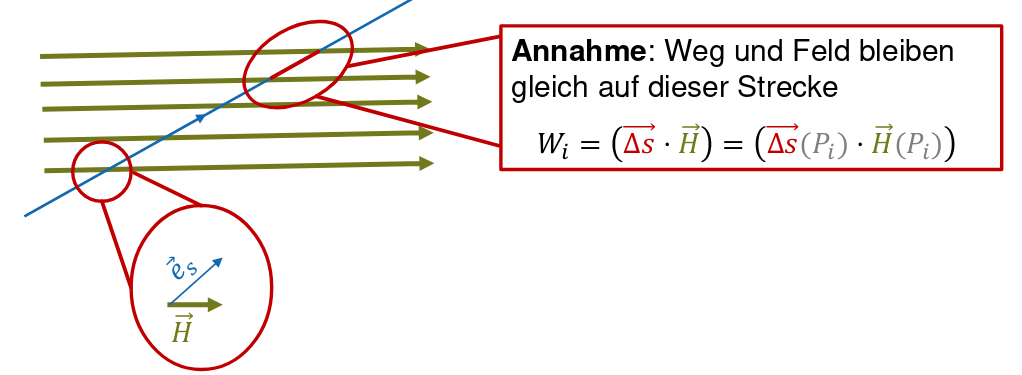
\includegraphics[scale=1.5]{img/wegintegral_beg.png}}
Die Arbeit $W_i$ bezeichnen wir als die Arbeit, welche wir aufwenden müssen, um uns auf dem Weg $\gamma$ um ein Stück $\Delta s$ nach Vorne zu bewegen. \\
Diese Arbeit ist Abhängig davon, wie Weg und Feld geometrisch stehen. Möchten wir uns senkrecht zum Feld bewegen, so wirkt nichts dieser Bewegungsrichtung entgegen und die  Arbeit ist gleich 0. \\
Möchten wir uns hingegen parallel zum E-Feld bewegen, so müssen wir maximale Arbeit verrichten, da das E-Feld uns maximal beeinflusst. \\
\\
Den Winkel, welcher das Feld mit dem Weg einschliesst, ist gegeben als $ cos(\varphi) = \vec{e}_s \cdot \vec{e}_H$. \\
Somit gilt für die Arbeit, welche auf dem Weg $\Delta s$ aufgewendet wird: $W_i = |H(P_i)| \cdot \Delta s \cdot  \vec{e}_s \cdot \vec{e}_H = \vec{H}(P_i) \cdot \Delta \vec{s}(P_i)$ \\
Für den gesamten Weg gilt somit:
$\displaystyle W_{ges} = \sum_i W_i = \sum_i \vec{e}_H = \vec{H}(P_i) \cdot \Delta \vec{s}(P_i) \Rightarrow i\rightarrow \infty $

\begin{center}
	$ W_{ges} = \int_A^B \vec{H}(\vec{P})\cdot d\vec{s} $
\end{center}
Ist der Weg s als Funktion gegeben, mit $s(t_0) = A $ und $s(t_e) = B$, so gilt für den Punkt P: $\vec{P} = \vec{s}(t)$ und den kleinen Richtungsvektor $ d\vec{s}$  des Weges: \\


\fboxsep=0pt
\begin{minipage}[t]{0.68\linewidth}

	\begin{flushright}
		$ \vec{s}(t) = \left(\begin{array}{c} f_1(t) \\ f_2(t)  \end{array}\right)$ \\
		\fspace
		$ \displaystyle \frac{d}{dt}(\vec{s}(t)) = \dot{\vec{s}}(t) $ \\
		\fspace
		$ \displaystyle d\vec{s}(t) = \dot{\vec{s}}(t) \cdot dt = \left(\begin{array}{c} \dot{f}_1(t) \\ \dot{f}_2(t)  \end{array}\right) \cdot dt	$
	\end{flushright}
\end{minipage}
\hfill%
\begin{minipage}[t]{0.28\linewidth}
	\begin{flushleft}
$ \displaystyle \big | \ \ \  \frac{d}{dt} \big ( . \big ) $ \\

\fspace
\fspace
\fspace
$\displaystyle  \big |\ \  \cdot dt$ \\

\end{flushleft}
\end{minipage}


\begin{center}

\end{center}



Und somit für das gesamte Integral: \\
\begin{center}
	$ \displaystyle \int_A^B \vec{H}(\vec{P})\cdot d\vec{s} = \int_{t_0}^{t_e} \vec{H}(\vec{s(t)})\cdot \dot{\vec{s}}(t) \cdot dt $
\end{center}
\iend


\bsptask{Beispiel}{Wegintegral über ein Vektorfeld}
\beginbsp
Gegeben sei das Vektorfeld in den Kartesischen Koordinaten $\vec{E}(x,y,z) =  \left(\begin{array}{c} x + 2y \\ 5z\\ x\\ \end{array}\right) $ \\
Berechnen sie das Wegintegral, über eine Gerade vom Punkt $\left(\begin{array}{c} 0 \\ 0\\ 0\\ \end{array}\right)$ zu $\left(\begin{array}{c} 5 \\ 2\\ 1\\ \end{array}\right)$
\iend

\vspace \fill

\bsp{Lösung}{}
\beginbsp
Zuerst müssen wir die Gerade vom Punkt $(0,0,0)$ zu $(5,2,1)$ als Funktion parameterisieren. \\
Aus der Vektorrechnung folgt für die Geradengleichung:
\begin{center}
	$\gamma(t) = \left(\begin{array}{c} 0 \\ 0\\ 0\\ \end{array}\right)  +  \left(\begin{array}{c} 5 \\ 2\\ 1\\ \end{array}\right) \cdot t = \left(\begin{array}{c} x \\ y\\ z\\ \end{array}\right)$
\end{center}
Somit gelten für Anfang und Endpunkte unserer Kurve:
\begin{center}
	$A = (0,0,0)^T = \gamma(0) \rightarrow t_0 = 0$ \\
	$B = (5,2,1)^T = \gamma(1) \rightarrow t_e = 1$
\end{center}

Für $d\vec{\gamma}$ folgt:
\begin{center}
	$ \displaystyle d\vec{\gamma} = \dot{\gamma} \cdot dt = \left(\begin{array}{c} \frac{d}{dt}(5 \cdot t) \\ \frac{d}{dt}(2 \cdot t)\\ \frac{d}{dt}(1 \cdot t)\\ \end{array}\right) \cdot dt = \left(\begin{array}{c} 5 \\ 2\\ 1\\ \end{array}\right) \cdot dt$
\end{center}

Und für $\vec{E}(\vec{\gamma}(t))$ :
\begin{center}
	$\vec{P} = \vec{\gamma(t)} =  \left(\begin{array}{c} 5t \\ 2t\\ 1t\\ \end{array}\right) = \left(\begin{array}{c} x \\ y\\ z\\\end{array}\right)$ \\
	$\Rightarrow \vec{E}(\vec{P}) =  \left(\begin{array}{c} 5t + 2\cdot2t \\ 5\cdot 1t\\ 5t\\ \end{array}\right) =  \left(\begin{array}{c} 9t \\ 5t\\ 5t\\ \end{array}\right) $ \
\end{center}
Somit folgt für das Integral:
\begin{center}
	$\displaystyle \doubleunderline{\int_\gamma \vec{E}\cdot d\vec{\gamma}} =  \int_0^1 \left(\begin{array}{c} 9t \\ 5t\\ 5t\\ \end{array}\right)  \cdot \left(\begin{array}{c} 5 \\ 2\\ 1\\ \end{array}\right)\cdot dt = \int_0^1 45t + 10t + 5t \cdot dt = \int_0^1 60t \cdot dt = \doubleunderline{30} $
\end{center}

\iend

\newpage

\bsptask{Beispiel}{Wegintegral in Kugelkoordinaten}
\beginbsp
Gegeben sei das Vektorfeld in Kugelkoordinaten $\vec{E}(r,\theta,\varphi) =  \left(\begin{array}{c} 5 \cdot r^2 \\ 0 \\ 0 \end{array}\right) = 5 \cdot r^2\cdot \vec{e}_r$ \\
Berechnen sie das Wegintegral, über eine Gerade (in Kugelkoordinaten) vom Punkt $\left(\begin{array}{c} 0 \\ 0\\ 0\\ \end{array}\right)$ zu $\left(\begin{array}{c} 5 \\ 0\\ 0 \\ \end{array}\right)$

\iend


\vspace \vfill
\bsp{Lösung}{}
\beginbsp
\textbf{Intuitive Lösung:} \\
Da der Weg parallel zum Feld ist ($\vec{e}_\gamma = \vec{e}_E$) vereinfacht sich das Wegintegral zu einem Skalaren Integral:
\begin{center}
	$\displaystyle \int_\gamma \vec{E}\cdot d\vec{\gamma} = \int_0^5 5 \cdot r^2 dr = \frac{1}{3} \cdot 5 \cdot 125 = \frac{625}{3}$
\end{center}
\textbf{Mathematische Lösung} \\
Wir beschreiben die Kurve $\gamma$ in Kugelkoordinaten:
\begin{center}
	$\gamma(t) = 5 \cdot t \cdot \vec{e}_r$
\end{center}
Somit folgt für $d \vec{\gamma}$
\begin{center}
	$d \vec{\gamma} = 5\cdot \vec{e}_r \cdot dt$
\end{center}
Und für das Integral:
\begin{center}

	$\displaystyle \int_\gamma \vec{E}\cdot d\vec{\gamma} =\int_0^1 \vec{E} \cdot 5 \cdot \vec{e}_r =  \int_0^1 5 \cdot (5t)^2 \cdot \vec{e_r} \cdot 5 \cdot \vec{e}_r dt =  \int_0^1 5^4 \cdot t^2 dt = \frac{1}{3} \cdot 5 \cdot 125 = \frac{625}{3}$
\end{center}
\iend

\newpage

\gl{Gleichung}{Fluss eines Vektorfeldes}
\begingl
Die folgende Gleichung bezeichnen wir als Oberflächenintegral des Vektorfeldes $\vec{E}$. \\
 Der Wert des Integrales gibt uns eine Information darüber, wieviel Feld durch eine gegebene Hüllfäche "fliesst" \\

\formulaBegin
$ \displaystyle \Phi = \oiint_A \vec{E} \cdot d\vec{A}$
\formulaEnd
\textbf{Variablen} \\
$\vec{E} =$ ein Vektorfeld\\
$A = $ Fläche, welche geschlossen ist\\
$\vec{A} =$ Normalenvektor der Fläche \\
\\

Das Integral selbst ist relativ schwer zu rechnen. Häufig lässt es sich jedoch vereinfachen:
Steht das Vektorfeld \textbf{senkrecht} zur Hüllfläche und ist es auf der gesamten Fläche \textbf{konstant}, so gilt für das Integral: \\

\formulaBegin
$ \displaystyle \oiint_A \vec{E} \cdot d\vec{A} = \pm A_{eff} \cdot |\vec{E}|$
\formulaEnd
\textbf{Variablen} \\
$A_{eff} =$ Die Fläche auf der das Feld ungleich 0 ist\\


Ist das Feld zwar konstant auf der gesamten Fläche, fliesst jedoch \textbf{nicht senkrecht} hindurch, so lässt sich das Integral auch zu einer Multiplikation vereinfachen:
\begin{center}
	\ibox{\includegraphics[scale=0.4]{img/vektorfIeld_oi.png}}
\end{center}
\formulaBegin
$ \displaystyle \oiint_A \vec{E} \cdot d\vec{A} = \pm A_{eff} \cdot |\vec{E}| \cdot cos(\varphi)$
\formulaEnd

\textbf{Variablen} \\
$\varphi =$ Winkel zwischen Vektorfeld und Flächennormale\\
\iend


\newpage


\bsptask{Beispiel}{}
\beginbsp
Wir betrachten ein Rohr der Länge L und mit Radius R. \\
In der Mitte des Rohres im Ursprung des Koordinatensystems befindet sich eine Wasserquelle, welche eine gewisse Menge Wasser generiert. \\
Die Flussdichte des Wassers, ist durch folgendes Vektorfeld gegeben: \\
\begin{center}

	$\displaystyle  \vec{J}_{wasser}(x,y,z) = \left\{
	\begin{array}{@{}l@{\thinspace}l}
		1 \cdot \vec{e}_y  \cdot [\frac{L}{s \cdot m^2}] & :  (x^2 + z^2) \leq R, y > 0 \\
			-1 \cdot \vec{e}_y  \cdot [\frac{L}{s \cdot m^2}] & :  (x^2 + z^2) \leq R, y \leq 0 \\
		0 \cdot \vec{e}_y  \cdot [\frac{L}{s \cdot m^2}] & : sonst                                                   \\
	\end{array}
	\right ) $
\end{center}

\begin{enumerate}
	\item  Zeichne das Vektorfeld in einem 3-Dimensionalen Koordinatensystem. \\
	\item Berechne sie das Oberflächenintegral $ \oiint_A \vec{J} \cdot d\vec{A}$ nach aussen, wobei A die Oberfläche des Rohres mit den beiden Kreisen am Ende bezeichne.
\end{enumerate}
\iend

\newpage

\bsp{Lösung}{}
\beginbsp
\begin{enumerate}
	\item  \
	\begin{center}

	      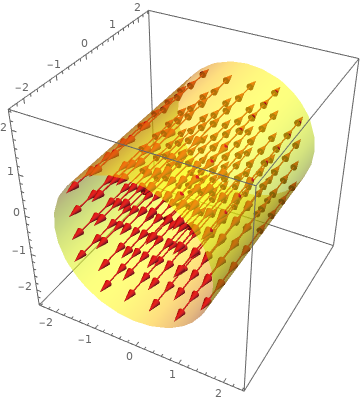
\includegraphics[scale=0.4]{plot.png}
	      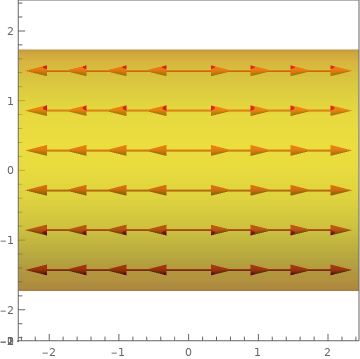
\includegraphics[scale=0.3]{plot2.png}

			\end{center}
	\item \textbf{Intuitiver Weg} \\
	Da das Vektorfeld nur auf den Kreisflächen ungleich Null ist, müssen wir nur das Oberflächenintegral über diese Kreisflächen berechnen. \\
	Da das Vektorfeld auf den Kreisflächen senkrecht steht und konstant ist, vereinfacht sich dieses Integral zu einer Multiplikation mit der Fläche: \\
	\begin{center}
			$\oiint_A \vec{J} \cdot d\vec{A} = A_{eff} \cdot |\vec{J}| = 2 \cdot (\pi R^2) \cdot 1 =  \doubleunderline{2\pi R^2}$
	\end{center}



	\textbf{Mathematischer Weg} \\ \begin{center}
		$\oiint_A \vec{J} \cdot d\vec{A} = \iint_{Mantel} 0 \cdot d\vec{A} + \iint_{Kreise} \vec{J} d\vec{A}$ \\
	\end{center}

		Wir bezeichnen nun mit $K_1$ die erste Kreisfläche des Zylinders bei $y = - \frac{L}{2}$ und mit $K_2$ die zweite Kreisfläche bei $y = \frac{L}{2}$. Somit folgt für das Integral:
		\begin{center}
		$\oiint_A \vec{J} \cdot d\vec{A} =  \iint_{K1} -1 \vec{e_y} \cdot  d\vec{A} + \iint_{K2} 1 \vec{e_y} \cdot d\vec{A}$
	\end{center}
	Die Flächennormalen auf der ersten Kreisfläche zeigt nach $(-e_y)$, die der 2. Kreisfläche nach $(e_y)$:
	\begin{center}
		$K_1$: $ d\vec{A} = (-\vec{e}_y) \cdot dA$, $K_2$: $ d\vec{A} = \vec{e}_y \cdot dA$ \\
		$ \rightarrow  \oiint_A \vec{J} \cdot d\vec{A} =  \iint_{K_1} -1 \vec{e_y} \cdot (- \vec{e_y})  dA + \iint_{K_2} 1 \vec{e_y} \cdot \vec{e_y} dA $ \\
		$ = 1\cdot \iint_{K_1} dA + 1\cdot \iint_{K_2} dA = \pi\cdot R^2 + \pi\cdot R^2 = 2 \cdot \pi\cdot R^2$

	\end{center}

\end{enumerate}

\iend
